\section{Introduction}
\cut{%%%%%%%%%%
Data-driven approaches employ machine learning to make use
of dependency treebank
and build up statistical models to deal with new sentences.
They outperform grammar-based
ones in that they free us from the labor to build
highly language-dependent rules
manually and adapt to our extension to everyday languages.
The two main solutions in
data-driven dependency parser hold quite different views and both gain fruitful results.
Graph-based approaches assign a score to a dependency tree by summing up the scores of
smaller fractions, and parsing is the process to find the candidate tree with highest score.
Graph-based decoders borrow algorithms in graph theory to generate the dependency tree.
In contrast, transition-based approaches regard the parser as a transition system, and they take various actions
to build the dependency tree stepwise.
}%%%%%%%%%

Existing data-driven dependency parsers are divided into two classes,
graph-based and transition based. MSTParser\cite{mcdonald2005non},
%\footnote{http://www.ryanmcd.com/MSTParser/MSTParser.html}
a typical graph-based parser, utilizes an arc-factored score model
learned from the corpus, and uses dynamic programming
to find a maximum spanning tree as the final output.
MSTParser and its variants currently enjoy high accuracy
at some cost of parsing time.
However, such exact inference approach limits
the range of features that can be extracted\cite{mcdonald2007characterizing}.
Furthermore, to do high order non-projective parsing, MSTParser
first constructs a projective parse tree,
and then rearranges the edges in the tree\cite{mcdonald2006online}, which further adds
to the time cost.


MaltParser~\cite{nivre2003efficient}, which is the most representative of
%~\footnote{http://www.maltparser.org/},
transition-based parsers, carries out a sequence of actions
determined by a classifier trained from parsing sequences.
Because this process is strictly monotonic and greedy,
MaltParser is known to be very fast.
%MSTParser learns a score model from the corpus, while
%MaltParser trains a transition classifier from the converted oracle instances.
%However, both approaches have limitations, especially for
%parsing non-projective languages~\cite{mcdonald2007characterizing}.
%The dynamic programming framework, while producing exact best solution,
%limits
Transition based parsers tend to establish arcs between two words only
when the words between them in the sentence have already been processed.
In other words, parsing is done incrementally by processing
smaller word spans into subtrees first before combining smaller subtrees
into bigger ones. Consequently, MaltParser has not met much success with
non-projective parsing.\footnote{The later proposal of SWAP action
ameliorate some of this problem. But training a classifier for this
action is hard due to limited resources of training data.}


%For MaltParser, the greedy decision-making gives rise to the
%error propagation. It imposes the restriction that an arc must be built
%between the top word of the stack and the next word in the input buffer.
%This is the main cause of a low accuracy on non-projective parsing
%in MaltParser, because predicting the SWAP actions correctly is
%rather important.
%\KZ{Don't understand the following sentence. You haven't pointed out the problems with MST and Malt clearly.}
%Moreover, how about comparing these two parsing process with our behavior?


%\KZ{Rephrase the following paragraph. It's too casual.
%Also what is the benefit of doing this over the malt and mst
%approach? It's not obvious.}


Studies in psycholinguistics revealed more about human comprehension for sentence. Given a sentence, humans are likely to first perform a rapid, shallow recognition of major phrases and then derive a complete parse, based on the quick analysis for phrases.\cite{townsend2001sentence} This provides us with an intuition that we can deal with the easiest relations first and incorporate the already built structures for later parse. 
This idea was simply employed by easy-first parser presented at 2010.\cite{goldberg2010efficient} However, due to the transition-based method, the parsing decision is still quite local and it is not so effective on non-projective sentence.
%
%\YZ{The following paragraph needs modification.}When parsing natural language, human beings neither exhaustively try out every possible sub-trees like MSTParser,
%nor take shift-reduce like actions as MaltParser.
%Instead, we scan through the sentence and simplify the sentence structure
%by folding modifiers under their head words.
%%, which is similar to the operations on stack and input buffer in MaltParser.
%In this process, we either find the head for the current word from the
%remaining words directly or
%delay its processing until it's easier to locate the candidates when the
%sentence structure becomes simpler.
%%As for head mapping, we may consider from both syntactic and semantic view to choose a proper head.

%\BF{explain 'sequence'}
This paper demonstrates a parsing framework that follows the above
intuition. It has two key components: the {\em sequence predictor}
generates a permutation of words in the input sentence,
which represents the sequence in which the words should be processed;
the {\em head mapper} takes each word from the
sequence and looks for its head in the unprocessed words, and marks it as processed.
Sequence predictor guides the parser to process
the simplest and most confident word in current state while
head mapper conducts search for the head of that word.
This framework can be seen as a natural union of transition-based
with graph-based parsers. On one hand, it is greedy and monotonic in
that processed words will not be processed again; on the other hand,
all graph-based search techniques (including 1st order and high order
features) can be applied in the head mapping process.

The main contributions of this work are:
%\begin{enumerate}
% \setlength{\itemsep}{0pt}
%  \item Proposing a novel and flexible dependency parsing framework.
%  \item Unifying the decoder for both projective and non-projective cases.
%  \item Presenting some interesting intermediate experiments and results on the study of sequence.
%  \item Our current best system combines graph-based parser and transition-based parser in an original way,
%  \BF{which provides a higher accuracy than MaltParser and parses faster than MSTParser.}
%\end{enumerate}
i) we propose a novel and flexible sequence-based dependency parsing framework;
ii) the framework includes a unified decoder for both projective and
non-projective languages (unlike MSTParser that requires the knowledge of
the input language in advance);
%iii) we present some interesting intermediate experiments and results on the study of parsing sequences; and
iii) our system shows promising results in both accuracy and speed.
%\BF{which provides a higher accuracy than MaltParser and parses faster than MSTParser.}
%\KZ{What's the advantage of combining the two approaches?
%List your contributions here.}
\begin{figure*}[th]
\centering
\epsfig{file=sysoverviewgrapheps.eps, width=1.8\columnwidth}
\caption{BeanParser Framework}
\label{fig:workflow}
\end{figure*}
